\documentclass[mathNotesPreamble]{subfiles}
\begin{document}
%\relscale{1.4}
\section{3.6: Rate of Change Applications}
\begin{defn*}[Average and Instantaneous Velocity]
  Let $s=f(t)$ be the position function (sometimes referred to as the \textbf{displacement} function) of an object moving along a line. The \textbf{average velocity} of the object over the time interval $\sbrkt{a,a+\Delta t}$ is the slope of the secant line between $\parens{a,f(a)}$ and $\parens{a+\Delta t,f(a+\Delta t)}$:
    $$v_{avg}=\frac{f(a+\Delta t)-f(a)}{\Delta t}$$
  
  The \textbf{instantaneous velocity} at $a$ is the slope of the line tangent to the position curve, which is the derivative of the position function:
    $$v(a)=\lim_{\Delta t \to 0} \frac{f(a+\Delta t)-f(a)}{\Delta t}=f'(a).$$
\end{defn*}
\vspace*{\stretch{1}}

\begin{ex*}[Position and velocity of a patrol car]\ 

\noindent
Assume a police station is located along a straight east-west freeway. At noon ($t=0$), a patrol car leaves the station heading east. The position function of the car $s=f(t)$ gives the location of the car in miles east $(s>0)$ or west $(s<0)$ of the station $t$ hours after noon.
\end{ex*}
\vspace*{-20pt}
\begin{minipage}[t]{0.6\linewidth}\ 

  \begin{tasks}(1)
    \task Describe the location of the patrol car during the first 3.5hr of the trip.
    \task Calculate the displacement and average velocity of the car between 2:00 P.M. and 3:30 P.M. 
    
    $(2\leq t\leq3.5)$.
    \task At what time(s) is the instantaneous velocity greatest \textit{as the car travels east}?
  \end{tasks}
\end{minipage}%
\begin{minipage}[t]{0.4\linewidth}\ 

  \begin{flushright}
    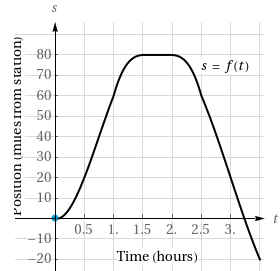
\includegraphics[width=0.85\linewidth]{images/fig3-40}
  \end{flushright}
\end{minipage}

\pagebreak
\begin{defn*}[Velocity, Speed, and Acceleration]
  Suppose an object moves along a line with position $s=f(t)$. Then
    \begin{center}
      \def\arraystretch{2}
      \begin{tabular}{@{}lR@{\ =\ }L@{}}
        the \textbf{velocity} at time $t$ is& v& \dfrac{ds}{dt}=f'(t)\\
        the \textbf{speed} at time $t$ is & \abs{v}&\abs{f'(t)}, \text{ and}\\
        the \textbf{acceleration} at time $t$ is & a&\dfrac{dv}{dt}=\dfrac{d^2s}{dt^2}=f''(t).
      \end{tabular}
    \end{center}
\end{defn*}
\noindent
\begin{minipage}[t]{0.6\linewidth}~
  \begin{itemize}
    \item Velocity indicates direction: 
    
    \hfill forward is positive, backward is negative
    \item Speed is direction independent:
    
    \hfill $v(t)=-30 m/s \Rightarrow \textnormal{speed }=30 m/s$.
    \item If displacement changes signs, then velocity was zero.
    
    A velocity of zero does not indicate a change in direction.
  \end{itemize}
\end{minipage}%
\begin{minipage}[t]{0.4\linewidth}~

  \begin{flushright}
    \begin{tikzpicture}
      \begin{axis}[
        axis lines=center,
        axis line style={->},
        xmin=-0.5, xmax=5.0,
        ymin=-7.5, ymax=22.5,
        xtick={-4,1,...,6},
        ytick={-5,5,...,25},
        minor x tick num=3,
        minor y tick num=1,
        ticklabel style={font=\footnotesize,inner sep=0.5pt,fill=white,opacity=1.0, text opacity=1},
        %xlabel=$x$, xlabel style={at={(ticklabel* cs:1)},anchor=north west},
        %ylabel=$y$, ylabel style={at={(ticklabel* cs:1)},anchor=south west},
        every axis plot/.append style={line width=0.95pt}
        ]
        \addplot[-] expression[domain=0:5, ClemsonOrange, samples=100] {x^3-6*x^2+9*x}
          node[above, black, pos=0.15] {$s$};
        \addplot[-] expression[domain=0:5, ClemsonPurple, samples=100] {3*x^2-12*x+9}
          node[right, black, pos=0.025] {$v$};
        \addplot[-] expression[domain=0:5, black, opacity=0.60, samples=2, text opacity=1] {6*x-12}
          node[above, black, pos=0.65] {$a$};
      \end{axis}
    \end{tikzpicture}
  \end{flushright}
\end{minipage}%

\pagebreak
\begin{ex*}
  $s=-t^3+3t^2-3t,\ 0\leq t\leq 3$ gives the position $s=f(t)$ of a body moving on a coordinate line, with $s$ in meters and $t$ in seconds.
  \begin{enumerate}
    \item Find the body's displacement and average velocity for the given time interval.
    \item Find the body's speed and acceleration at the endpoints of the interval.
    \item When, if ever, during the interval does the body change direction?
  \end{enumerate}
\end{ex*}

\pagebreak
\noindent
For vertical motion (e.g. an object thrown up in the air), an object's maximum height occurs when velocity is zero and hits the ground at height zero.
\begin{ex*}
  A rock is thrown vertically upward from the surface of the moon at a velocity of 24 m/sec (about 86 km/h) reaches a height of $s=24t-0.8t^2$ meters in $t$ sec.
  \begin{enumerate}
    \item Find the rock's velocity and acceleration at time $t$. (The acceleration in this case is the acceleration of gravity on the moon.)
    \item How long does it take for the rock to reach it's highest point?
    \item How high does the rock go?
    \item When does the rock hit the ground?
    \item What is the velocity at that instant?
  \end{enumerate}
\end{ex*}

\pagebreak
\begin{ex*}
  Suppose a stone is thrown vertically upward from the edge of a cliff on Earth with an initial velocity of 32 ft/s from a height of 48 ft above the ground. The height (in feet) of the stone above the ground $t$ seconds after it is thrown is $s(t)=-16t^2+32t+48$.
  \begin{enumerate}
    \item Determine the velocity $v$ of the stone after $t$ seconds.
    \item When does the stone reach its highest point?
    \item What is the height of the stone at the highest point?
    \item When does the stone strike the ground?
    \item With what velocity does the stone strike the ground?
    \item On what intervals is the speed increasing?
  \end{enumerate}
\end{ex*}

\pagebreak
\begin{ex*}[Velocity of a bullet]
  A bullet is fired vertically into the air at an initial velocity of 1200 ft/s. On Mars, the height $s$ (in feet) of the bullet above the ground after $t$ seconds is $1200t-6t^2$ and on Earth, $s=1200t-16t^2$. How much higher will the bullet travel on Mars than on Earth?
\end{ex*}

\pagebreak
\begin{defn*}[Average and Marginal Cost]
  The \textbf{cost function} $C(x)$ gives the cost to produce the first $x$ items in a manufacturing process. The \textbf{average cost} to produce $x$ items is $\bar C(x)=C(x)/x$. The \textbf{marginal cost} $C'(x)$ is the approximate cost to produce one additional item after producing $x$ items.
\end{defn*}
\begin{ex*}
  Suppose $C(x)=10,000+5x+0.01x^2$ dollars is the estimated cost of producing $x$ items. The marginal cost at the production level of 500 items is:
\end{ex*}
\vspace*{\stretch{1}}

\begin{ex*}
  The cost function for production of a commodity is
    $$C(x)=339+25x-0.09x^2+0.0004x^3$$
  \begin{enumerate}
    \item Find and interpret $C'(100)$.
    \item Compare $C'(100)$ with the cost of producing the 101st item.
  \end{enumerate}
\end{ex*}

\vspace*{\stretch{1}}
\pagebreak

\begin{ex*}
  For the following cost functions,
  \begin{enumerate}[label=\alph*)]
    \item Find the average cost and marginal cost functions.
    \item Determine the average cost and the marginal cost when $x=a$.
    \item Interpret the values obtained in part (b)
  \end{enumerate}
  \begin{enumerate}[itemsep=\stretch{1}]
    \item $C(x)=500+0.02x,\ 0\leq x\leq 2000,\ a=1000$.
    \item $C(x)=-0.01x^2+40x+100,\ 0\leq x\leq 1500,\ a=1000$.
  \end{enumerate}
  \vspace*{\stretch{1}}
\end{ex*}

\pagebreak
\end{document}
